\documentclass[../root.tex]{subfiles}

\begin{document}

\chapter{Introduction}
\section{Motivation}
\lettrine{S}{olving} optimization problems has become ubiquitous in robotics.
Nearly all of the recent breakthroughs in robotics have been enabled by solving 
optimization problems. Whether these are optimizing extremely large neural networks 
for better perception, finding an optimal alignment when fusing sensor data, calculating
the most probable map and location history from sensor data, or calculating the next 
command to send to a robot to achieve a pre-specified objective, solving optimization
problems reliably and efficiently has become central to many tasks across all stages of 
the autonomy pipeline. 

Many simple robots can be controlled effectively with classical control techniques 
such as proportional-integral-derivative (PID) control or linear-quadratic regulators (LQR);
however, as our robots become increasingly complex and as we demand increasing levels of autonomy, 
robustness, efficiency, and performance, the need for more advanced, optimization-based control 
techniques such as model-predictive control (MPC) has risen. 
Online optimization methods such as MPC, where small but descriptive optimization problems 
are solved in real time, have enabled many impressive achievements in recent years across
a breadth of applications, including aerospace, legged locomotion, autonomous driving,
and manipulation (see Fig. \ref{fig:applications}).

\begin{figure}[t]
    \centering
    \begin{subfigure}[b]{0.24\columnwidth}
        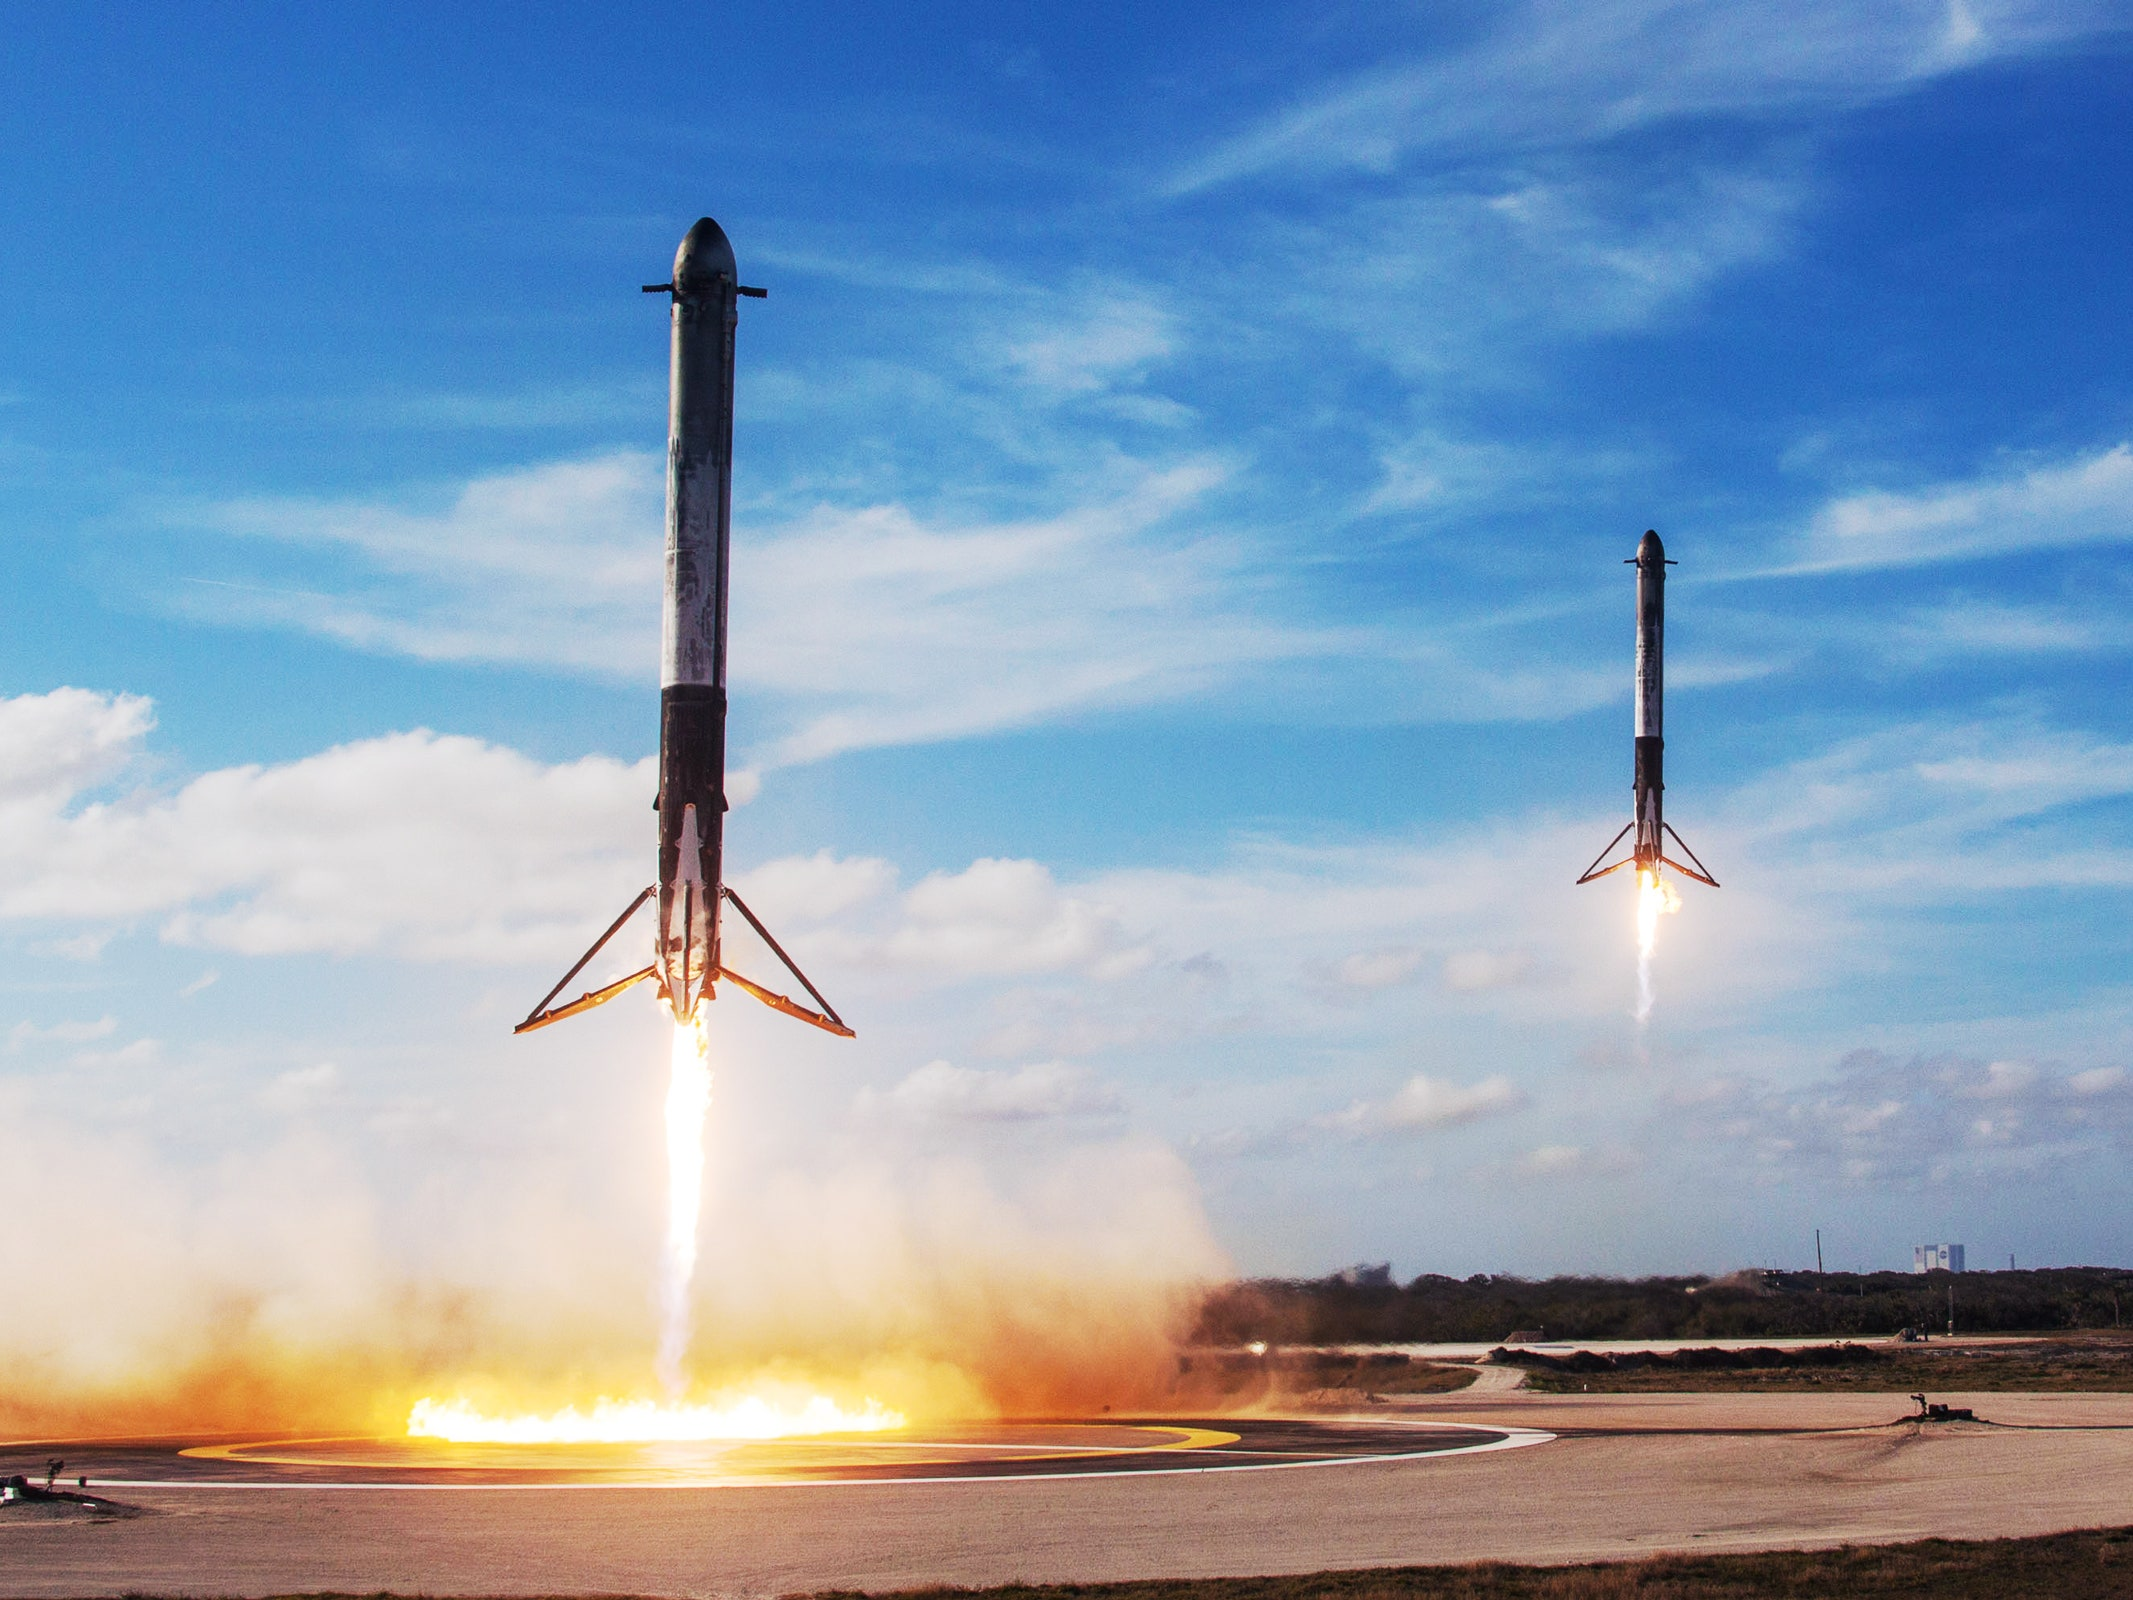
\includegraphics[height=0.8\textwidth, trim=3cm 0 3cm 0, clip]{spacexrocketreturn.jpg} 
        \caption{}
    \end{subfigure}
    \begin{subfigure}[b]{0.24\columnwidth}
        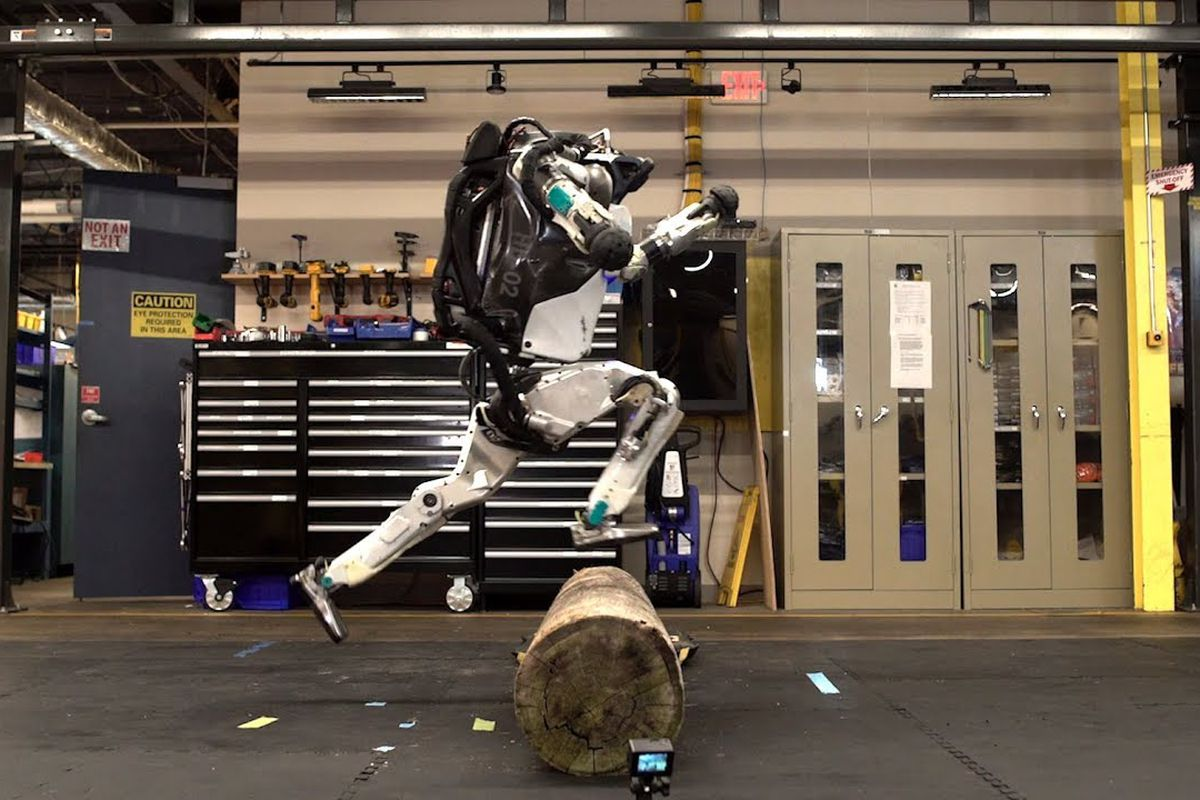
\includegraphics[height=0.8\textwidth, trim=4cm 0 4cm 0, clip]{atlas.jpg} 
        \caption{}
    \end{subfigure}
    \begin{subfigure}[b]{0.24\columnwidth}
        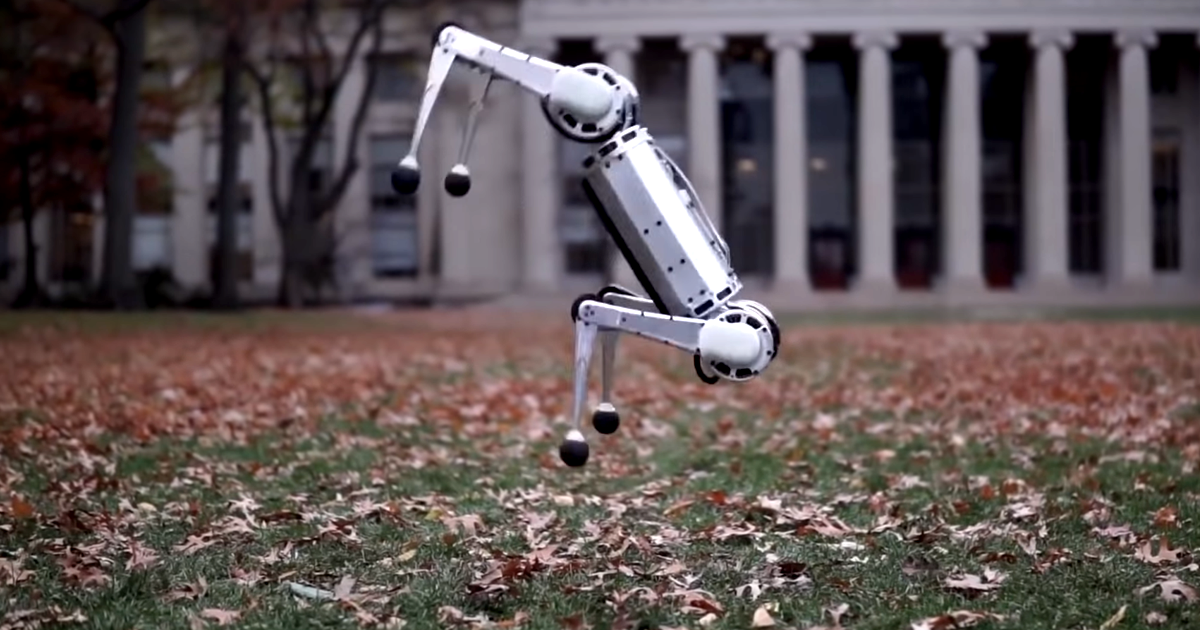
\includegraphics[height=0.8\textwidth, trim=8cm 0 8cm 0, clip]{mini-cheetah-robot-bloopers.png} 
        \caption{}
    \end{subfigure}
    \begin{subfigure}[b]{0.24\columnwidth}
        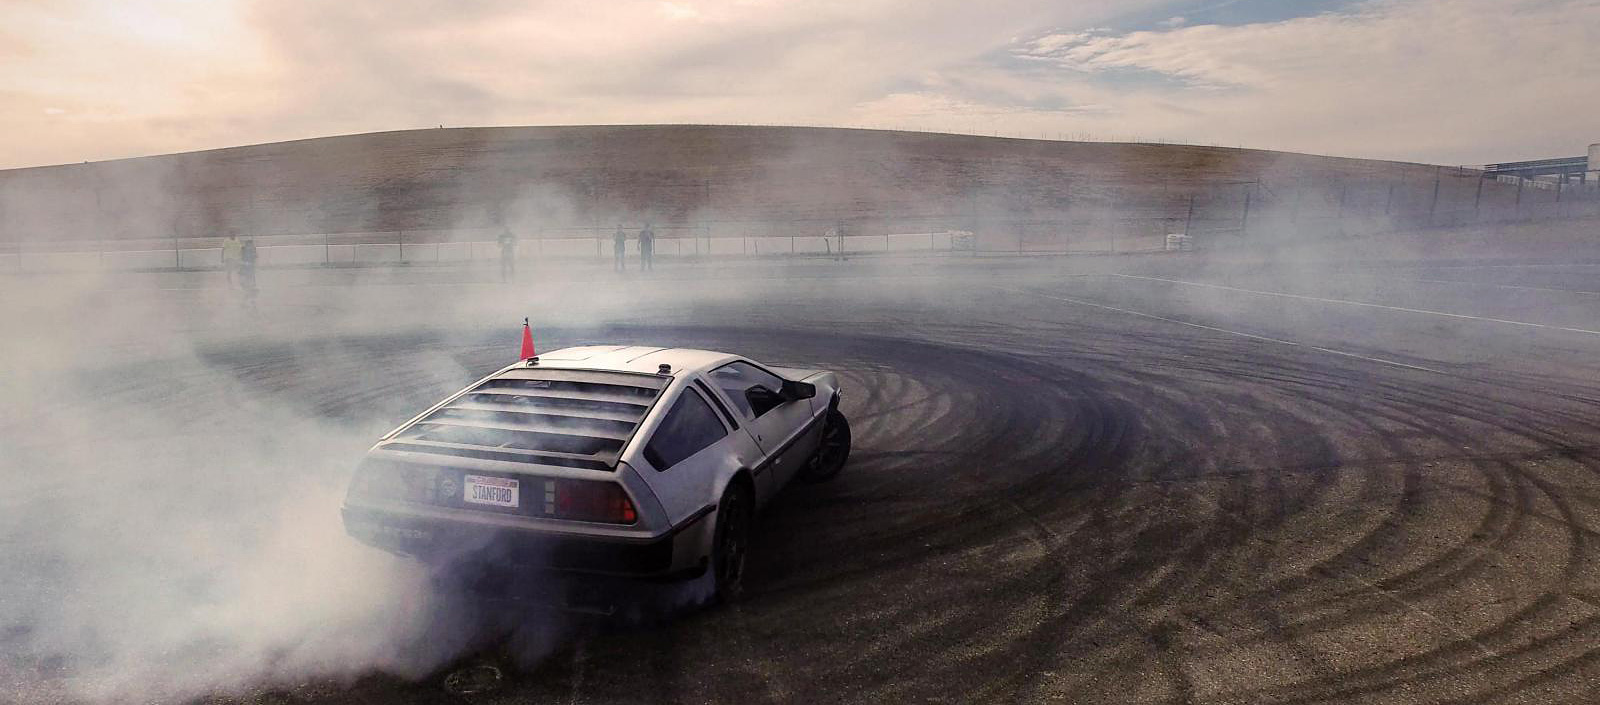
\includegraphics[height=0.8\textwidth, trim=100 0 400 0, clip]{Stanford_MARTY_005_remasted-banner.jpg} 
        \caption{}
    \end{subfigure}
    \caption{Notable recent successes of optimal control, a) SpaceX rocket
    booster landing (2018), b) Boston Dynamics' Atlas doing parkour (2018), c)
    MIT Mini Cheetah doing backflips (2019), and d) Stanford's MARTY drifing
    around a racecourse (2019).}
    \label{fig:applications}
\end{figure}

Trajectory optimization, a subset of the more general field of optimal
control, is a powerful and promising method for controlling complex robotic
systems. This general framework allows a user to specify a possibly-nonlinear
cost function encoding objectives such as distance to a goal, energy
consumption, smoothness, or time of arrival. A set of state and control
trajectories that minimize the objective while obeying the nonlinear and
generally underactuated system dynamics, in addition to any other constraints
such as joint or torque limits, obstacle avoidance, etc., is returned to the
user and sent to the robot.

Trajectory optimization can be used to generate trajectories for a wide
variety of systems, including aerial vehicles subject to complex nonlinear
aerodynamic forces, legged systems that make and break contact with their
environment, serial-link manipulators that interact physically with their
environment, or spacecraft trajectory design that finds low-cost orbit
transfers for trajectories spanning the coarse of days or even months. In
short, trajectory optimization can generate optimal motion plans for nearly
every robotic system we care about, while taking into account an extremely
wide variety of constraints or control objectives.

However, this generality and expressivity comes at the cost of significant
computation. The resulting nonlinear programs (NLPs) are constrained,
non-convex problems where finding the global minimum is almost always
computationally intractable. As a result, most methods rely on finding local
minima using gradient information from the objective and constraints. Solving
these problems reliably and efficiently remains an open problem in the field
of optimal control.

As a result, most modern control techniques rely on convex approximations of
these problems, whose global solution can be found reliably and generally in
bounded time. The full, nonlinear problem is often solved offline and used as a
reference for online control, sometimes in the form of a trajectory library.
However, these convex approximations often make limiting assumptions about the
problem or the system, limiting performance. The ability to solve the full
nonlinear trajectory optimization problem fast enough to do online replanning or
model-predictive control (MPC) has the potential to open up a new frontier of
performance for the next generation of robots. This could mean increased
capabilities and output for scientific exploration robots such as Mars rovers or
underwater robots exploring the depths of our oceans. Or it could lead to
increased operational regimes for legged locomotion, allowing these systems to
be incorporated in sectors such as healthcare, surveillance, last-mile delivery,
or inspection, all while increasing operation time and minimizing the need for
human intervention. To open up new frontiers of capabilities, the robots of
today and tomorrow need to have---among many other important 
capabilities---increased capacities to make decisions, generate plans, and move
efficiently through complex and uncertain environments. The ability to solve
planning and control problems in real time is one step to move us closer towards
that lofty goal.

The goal of this thesis is to develop faster and more reliable algorithms for
solving trajectory optimization problems, and demonstrate the performance
gains that can be realized by solving the full nonlinear trajectory
optimization problem in real time.

\section{Key Challenges} 

There are many challenges associated with developing state-of-the-art
optimization solvers. Simply finding the right algorithm for the task at
hand, one that performs reliably and efficiently, is a challenging task given
the seemingly infinite ways to assemble a good nonlinear optimization solver
\cite{nocedal_Numerical_2006}. Once a good algorithm has been found, it is
then another challenging step to implement it well enough in software to beat
other solvers, since memory management, numerical stability, and generality
all play critical roles, let alone implementing it in such a way that it can
be used or replicated by others. Since this is often a low priority for
academics, this makes comparisons against existing methods a challenge in
itself. Even when implemented, getting the algorithm to work on real
hardware instead of in simulation is another nontrivial task.

In short, developing novel optimization algorithms is a challenge, which is
why most roboticists use existing solvers rather than writing their own.
However, as demonstrated in this thesis, the performance gains obtained from
writing optimization methods developed for a particular application,
leveraging domain insight and problem structure, are almost always worth the
effort.

\section{Contributions}

Our contributions are:
\begin{enumerate}
    \item ALTRO, a state-of-the-art solver for constrained nonlinear trajectory 
    optimization written in Julia. Released open-source as part of a suite of 
    official packages for setting up and solving trajectory optimization problems,
    it offers state-of-the-art performance with a convenient, user-friendly API 
    and thorough documentation.
    \item ALTRO-C, an extension of the original ALTRO algorithm that handles
    second-order cone programs and offers state-of-the-art performance for
    both nonlinear and convex MPC problems problems. To the authors'
    knowledge, it is the first nonlinear trajectory optimization solver to
    natively handle conic constraints.
    \item A powerful and intuitive method for solving optimization problems with 
    3D rotations, based entirely on the approachable fields of matrix calculus
    and linear algebra.
    \item A novel parallel direct linear system solver for the KKT systems that 
    arise when solving trajectory optimization problems. 
    \item A scalable method for generating trajectories for teams of quadrotors
    carrying a single payload.
    \item A sample-efficient method for improving MPC controller performance by 
    combining information from an approximate prior model with data from the real 
    system.
\end{enumerate}

\section{Outline}

% TODO: Update this
In the following section we provide a survey of trajectory optimization and
optimal control, focusing on the work done in the last 20 years. Part
\ref{part:theory}, comprising Chapters
\ref{chap:altro}-\ref{chap:mctrajop}, focuses on our theoretical and
algorithmic contributions to the field of optimal control. In Chapter
\ref{chap:altro}, we provide an in-depth derivation of the ALTRO algorithm, along
with the benchmarks results obtained in 2018 and published in
\cite{howell_ALTRO_2019}. Chapter \ref{chap:altro_c} builds on this work,
describing extensions of the ALTRO algorithm to conic MPC problems,
demonstrating state-of-the-art performance on a variety of convex and conic MPC 
benchmark problems.
Chapter \ref{chap:attitude} details a powerful and intuitive methodology 
for solving optimization problems for systems with 3D rotations, and includes
details on adapting the ALTRO algorithm to natively handle unit quaternions. 
The following two chapters consider algorithms that are better-suited to 
leveraging parallel computation. Chapter \ref{chap:rslqr} proposes a novel method direct 
linear system that uses recursive Schur compliments to parallelize across the temporal 
domain. Chapter \ref{chap:mctrajop} focuses instead on the spatial domain, considering the
the feasibility of applying direct collocation in maximal coordinates using the Ipopt 
solver, where parallelization is natural exposed across each body of a multi-body 
system.

Part \ref{part:application} focuses on applications of the theoretical and 
algorithmic contributions of Part \ref{part:theory} to real systems. 
Chapter \ref{chap:distributed} describes a method for generating a 
motion plan for a team of quadrotors carrying a single, heavy load using 
distributed trajectory optimization. Each of the distributed components 
use ALTRO to solve the trajectory optimization problem. The method 
is demonstrated in hardware. The final chapter, Chapter \ref{chap:jdmd} addresses the 
case where the nominal dynamics model is insufficient, and introduces a technique to 
improve the tracking performance of convex MPC controllers by combining information from 
an approximate model with data from the real system. Preliminary results are provided 
in high-fidelity simulation environments. Concluding remarks are given in 
\ref{chap:conclusion}.


\section{Literature Review} \label{sec:lit_review}
The field of optimal control has a long and rich history, beginning predominantly in the 
1950s and 1960s with the advent of space exploration and computers. The progress of the field of 
optimal control has naturally been closely linked with progress in the field of optimization 
and numerical computation. For an excellent overview of the state of optimal control
and trajectory optimization up to the turn of the century, see Betts' seminal 1998 survey 
\cite{betts_Survey_1998}. 

Historically, trajectory optimization algorithms have been split into one of two categories:
indirect and direct. Indirect methods derive a set of first-order necessary conditions on the 
continuous-time problem formulation, employing the well-known Pontryagin's Minimum (or Maximum)
Principle and the calculus of variations to derive a set of first-order ordinary differential 
equations (ODEs) describing a two-point boundary-value problem (BVP). This BVP is then solved
using any one of a variety of methods. Direct methods, on the other hand, first discretize the 
problem into a finite set of time steps, often referred to as ``knot points.'' This ``transcribes''
the infinite-dimensional continuous-time optimal control problem in a finite-dimensional NLP that
can be solved using any of the general methods for NLPs. The classic distinction between these 
methods is summarized as follows:
\begin{itemize}
	\item Indirect methods: ``Optimize, then discretize.''
	\item Direct methods: ``Discretize, then optimize.''
\end{itemize}

Despite being more brittle and requiring analytical derivatives for every problem, indirect methods 
were used frequently in the aerospace industry for many years. However, as computers got faster and 
the field of nonlinear optimization grew more mature, the runtime performance gap narrowed, and direct
methods became the de-facto standard for optimal control, given their improved robustness, ability to 
easily handle generic constraints, and the fact that writing general-purpose solvers that could
handle a wide variety of vehicle models and mission scenarios was much more straightforward \cite{betts_Survey_1998}.

Since the early 2000s, nearly all practitioners in both aerospace and robotics use direct methods, 
with a few exceptions \cite{antony_Rapid_2017}. Given that indirect methods are rarely used in practice, 
we'll restrict our attention to the various direct methods for trajectory optimization, with an 
emphasis on the work done in the last 20 years. Most modern approaches to trajectory optimization 
can be placed in one of two categories: those based on differential dynamic programming (DDP), and
those based on direct transcription. Since DDP-based approaches can be derived as an indirect method, 
some practitioners refer to these as indirect methods while referring to those based on direct 
transcription as direct methods. 


Direct transcription is a broad category of algorithms that discretize the
state and input trajectories in time and relate the resulting finite set of
states and controls across all time steps as decision variables in an NLP,
with the nonlinear system dynamics imposed as equality constraints. Direct
collocation is by far the most common version of direct transcription,
originally introduced in 1987 by Hargraves and Paris
\cite{hargraves_Direct_1987}. The most traditional implementation of direct
collocation uses Hermite-Simpson integration, which fits third-order splines
on the state and cost trajectories, and a first-order hold on the controls.
Since the dynamics are imposed as constraints between adjacent time steps,
most implemenations of direct collocation use implicit integration methods
for the first-order ODEs describing the system dynamics, since these methods
often exhibit improved robustness and energy conservation behavior over the
more traditional explicit Runge-Kutta-style integrators. Betts' 2001 book
\cite{betts_Practical_2001} is an excellent overview of these methods in the
aerospace community. Another excellent resource for an introductory overview
of direct collocation, especially for the robotics community, is Matthew
Kelly's tutorial and accompanying MATLAB code \cite{kelly_Introduction_2017}.
Important recent work in the field of robotics includes several works that
came out of Russ Tedrake's lab at MIT around the 2015 DARPA robotics
challenge, where they demonstrated 1kHz control on a 34 degree of freedom
(DOF) humanoid using an active-set method that uses problem-specific
heuristics to pick the active set \cite{kuindersma_Efficiently_2014}. This
work then grew to include methods for ``contact-implicit'' trajectory
optimization, where the optimization algorithm is free to pick the number and
timing of contact interactions with the environment
\cite{posa_Direct_2014,posa_Optimization_2016,manchester_Variational_2017,
patel_ContactImplicit_2019}. Another interesting extension to direct
collocation provides improved tracking performance of the resulting
trajectory given bounded uncertainties or disturbances
\cite{manchester_DIRTREL_2017}. Along similar lines, Howell et. al combine
direct trajectory optimization, deterministic sampling, and policy
optimization to derive a computationally tractable method for generating
robust motion plans \cite{howell_Direct_2021}.

While the traditional methods for direct collocation rely on fitting
low-order polynomials between time steps, more recent methods have
investigated the use of fitting global polynomials to the entire trajectory,
referred to as \textit{orthogonal}, \textit{global}, or
\textit{pseudospectral} collocation. These methods exhibit exponential
convergence in the order of the polynomial, as long as the underlying problem
is sufficiently smooth. These methods have been successfully applied to
aerospace applications, with the most famous example being zero-propellant
orientation slews for the International Space Station around 2007
\cite{kang_Pseudospectral_2007}. The surveys by Rao
\cite{rao_Survey_,rao_Trajectory_2014} give a good overview of these methods.
Due to their smoothness requirements and more complicated implementation,
these methods have received very little attention in the robotics community.

In contrast to methods based on direct transcription that typically rely on
general-purpose NLP software such as SNOPT \cite{gill_SNOPT_2005}, Ipopt
\cite{wachter_Implementation_2006} or the Knitro solver by Artelys, DDP-based
methods solve for a locally-optimal feedback policy by optimizing only over
the controls, maintaining strict dynamic feasibility by simulating the system
forward using the locally-optimal feedback policy. DDP was originally
introduced in 1966 \cite{mayne_Secondorder_1966} but was mostly ignored until
the early 2000s when it was picked back up by the robotics community,
deriving the well-known iterative LQR (iLQR) algorithm
\cite{todorov_Generalized_2005}. Taking a Gauss-Newton approach, iterative
LQR avoids the expense of calculating the second-order derivatives of the
dynamics. Similar to most Gauss-Newton algorithms, iLQR tends to take more
iterations but converge in overall less time than DDP. While fast and
relatively easy to implement, the traditional DDP-based versions had no
ability to work with additional constraints beyond the dynamics constraints.
Many methods were proposed over the years, including solving QPs at each time
step to handle simple bounds on the inputs \cite{tassa_Controllimited_2014}
or more general nonlinear constraints \cite{xie_Differential_2017},
projection onto the linearized constraints \cite{giftthaler_Projection_2017},
or augmented Lagrangian methods \cite{plancher_Constrained_2017}. A
derivative-free variant based on the unscented Kalman filter from the state
estimation community was also proposed \cite{manchester_Derivativefree_2016}.
Most recently, the developers of the Pinocchio dynamics library
\cite{carpentier_Pinocchio_2019} proposed a DDP solver that uses augmented Lagrangian
methods to handle equality constraints, building off of previous work covered
in this thesis \cite{kazdadi_Equality_2021}.

An important follow-on to constrained DDP that has received some significant
attention is ``multiple-shooting DDP,'' which breaks up the trajectory into a
series of sub-trajectories with continuity constraints linking them together.
Similar to traditional multiple shooting methods, multiple shooting DDP
allows for varying amounts of dynamic infeasibility, and can have better
numerical conditioning. Parallelism is another key benefit, since each
sub-trajectory can be processed in parallel. Giftthaler et. al. derive a
family of such methods and demonstrate superior convergence for MPC problems
\cite{giftthaler_Family_2017}, but was restricted to only the Gauss-Newton
approximation, i.e. iLQR. The application of multiple shooting with full DDP
to aerospace problems was studied in a recent two-part paper out of
University of Texas, Austin
\cite{pellegrini_Multipleshooting_2020,pellegrini_Multipleshooting_2020a}.
While both of these leveraged parallelism on a multi-core CPU, impressive
performance gains have recently been demonstrated on other hardware
accelerators, including GPUs and FPGAs \cite{plancher_Performance_2020}.

Iterative LQR and its variants have seen wide adoption in the legged
locomotion community, in particular. Real-time whole-body control for the
HRP-2 Humanoid was demonstrated using iLQR in 2015, a major breakthrough for
the optimal control community \cite{koenemann_Wholebody_2015}. Since then,
several labs have published papers demonstrating the successful application
of variants of iLQR for quadupedal locomotion
\cite{farshidian_Efficient_2017,mastalli_Crocoddyl_2019,neunert_WholeBody_2018}.

\end{document}